\documentclass{article}

\usepackage{graphicx, xcolor}
\usepackage{amsmath, amssymb}

\usepackage[margin=1in]{geometry}

\def\hwtitle{Homework 2: Numerical Integration}
\def\hwauthor{Caden Gobat}
\def\hwdate{\today}

\usepackage{fancyhdr}
\lhead{\hwauthor}
\chead{\hwtitle}
\rhead{\hwdate}
\lfoot{\hwauthor}
\cfoot{}
\rfoot{\thepage}
\renewcommand{\footrulewidth}{0.4pt}
\pagestyle{fancy}

\author{\hwauthor}
\title{\hwtitle}
\date{\hwdate}

\begin{document}

\maketitle
\thispagestyle{fancy}

\section{Introduction}

foo

\section{Results}

\bigskip
\noindent{\bf Question 1}
\medskip

\begin{figure}[h]
    \centering
    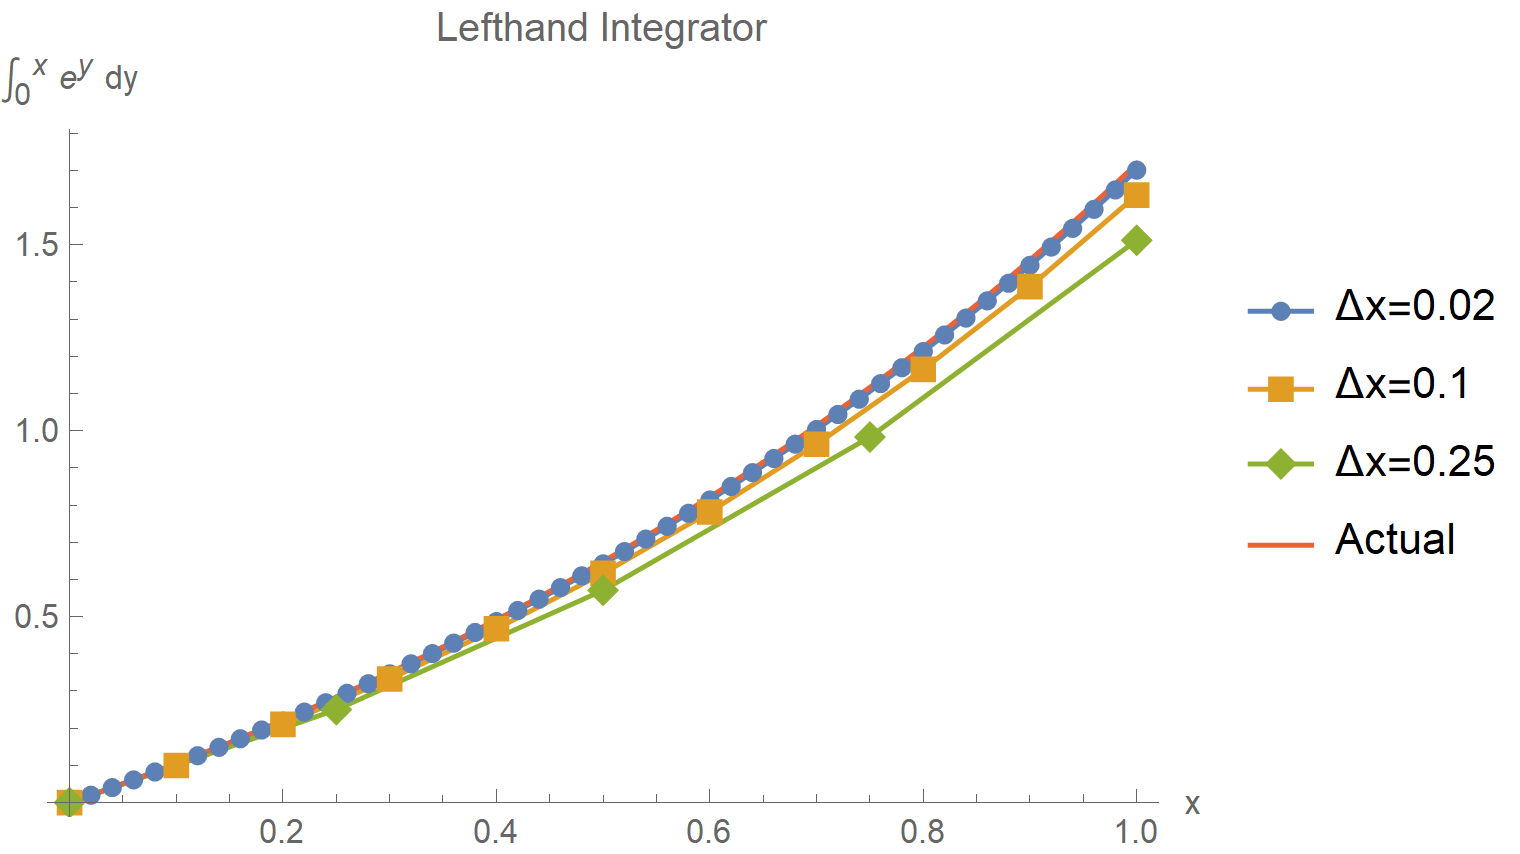
\includegraphics[width=5in]{homework2/P1_LH.png}
    \caption{Numerical integration results using the left-hand integrator formula for a variety of bin widths ($\Delta x$). The analytical result is plotted here as the line labeled ``Actual''.}
    \label{fig:p1_left}
\end{figure}

\begin{figure}[h]
    \centering
    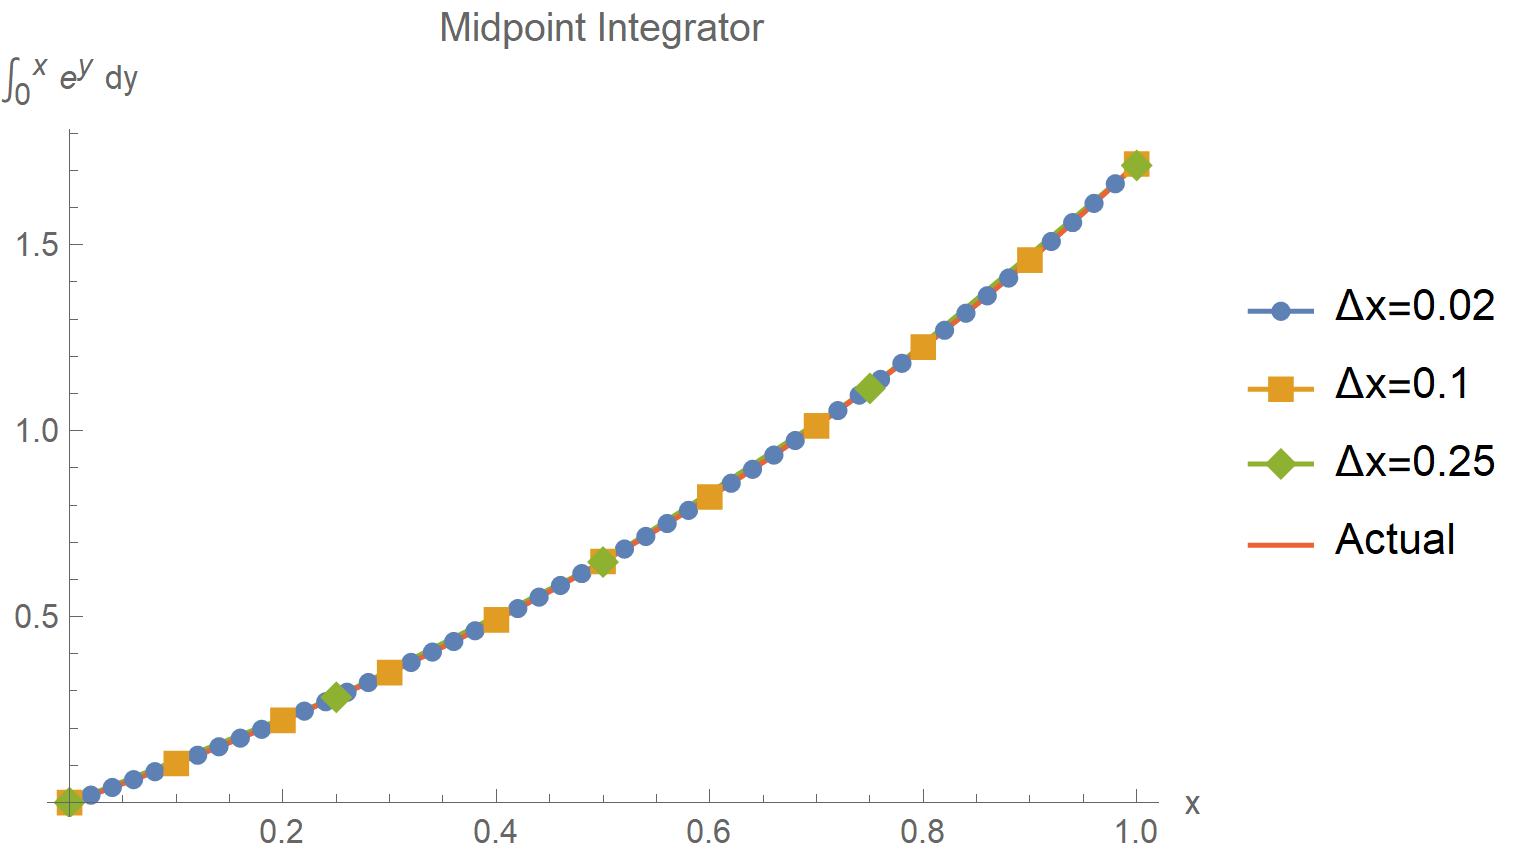
\includegraphics[width=5in]{homework2/P1_MP.png}
    \caption{Numerical integration results using the midpoint integrator formula for a variety of bin widths ($\Delta x$). The analytical result is plotted here as the line labeled ``Actual''.}
    \label{fig:p1_mid}
\end{figure}

\bigskip
\noindent{\bf Question 2}
\medskip

\begin{figure}[h]
    \centering
    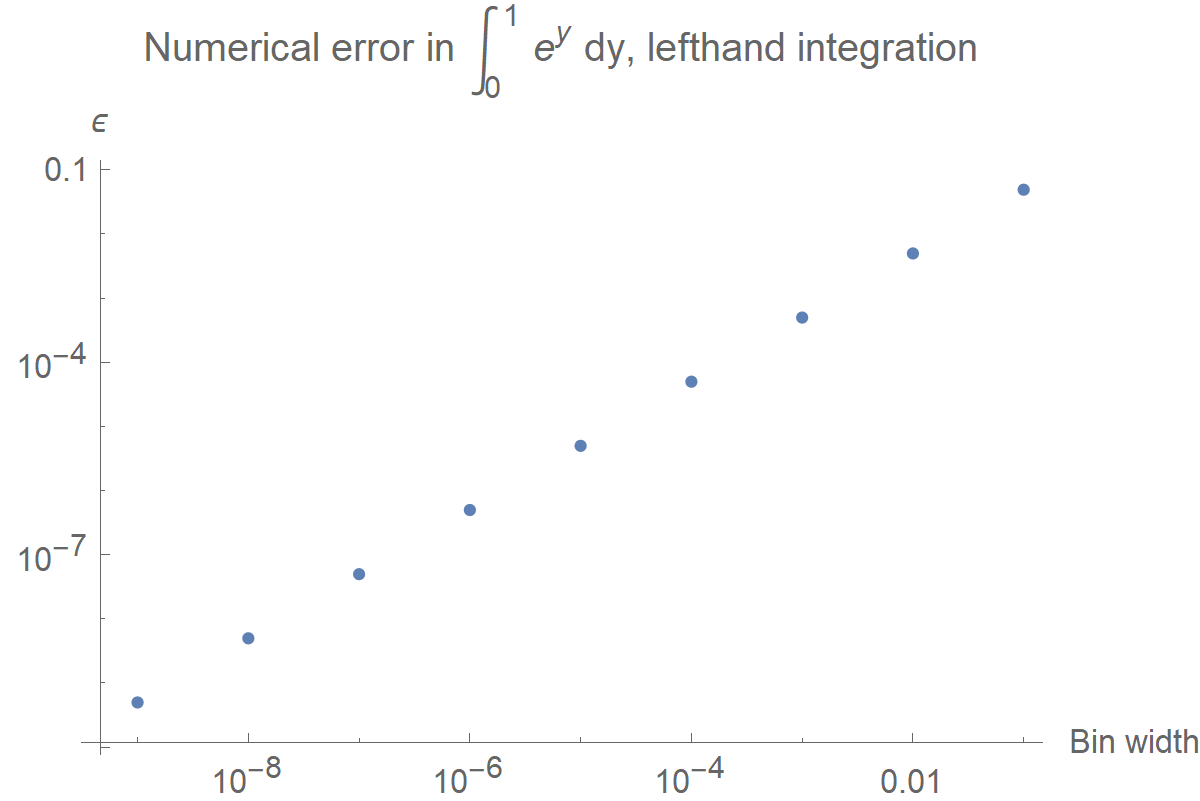
\includegraphics[width=5in]{homework2/P2.png}
    \caption{The slope is 0.999964}
    \label{fig:p2}
\end{figure}

\bigskip
\noindent{\bf Question 3}
\medskip

\begin{figure}[h]
    \centering
    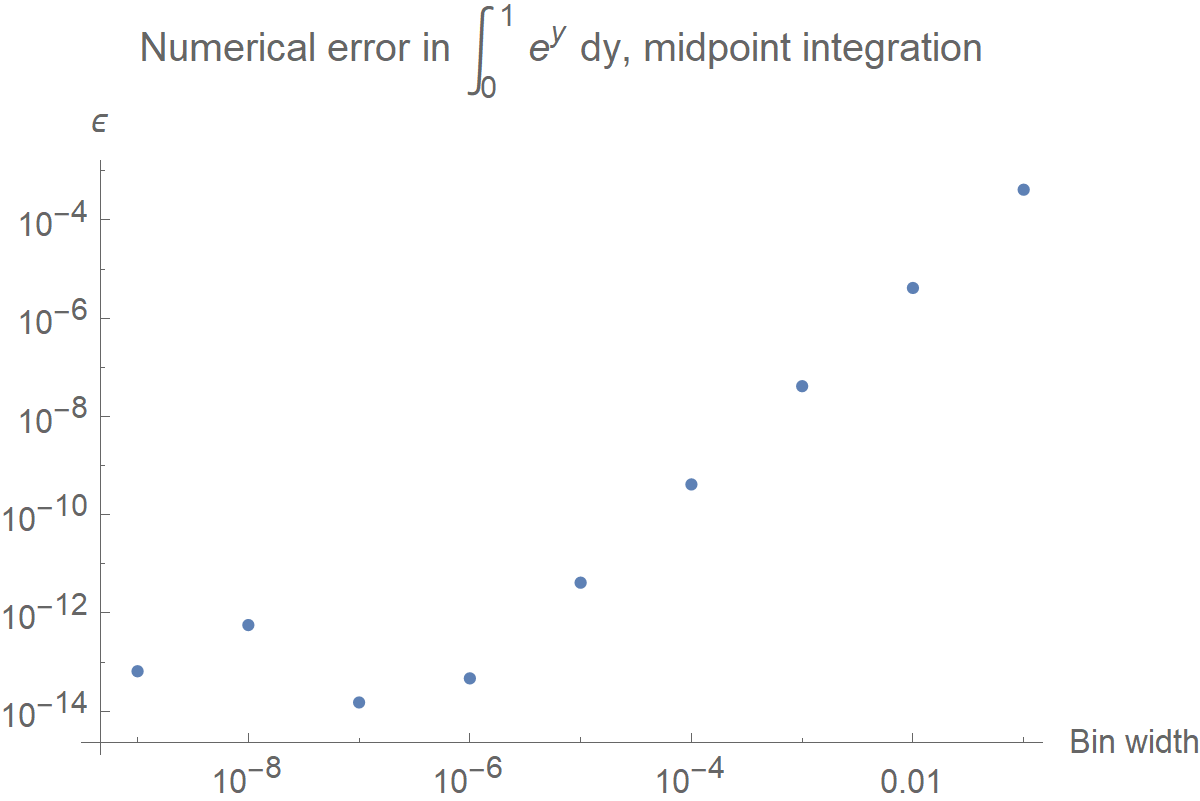
\includegraphics[width=5in]{homework2/P3.png}
    \caption{The slope is 1.99991}
    \label{fig:p3}
\end{figure}

\bigskip
\noindent{\bf Question 4}
\medskip


\bigskip
\noindent{\bf Bonus Question}
\medskip

\begin{figure}[h]
    \centering
    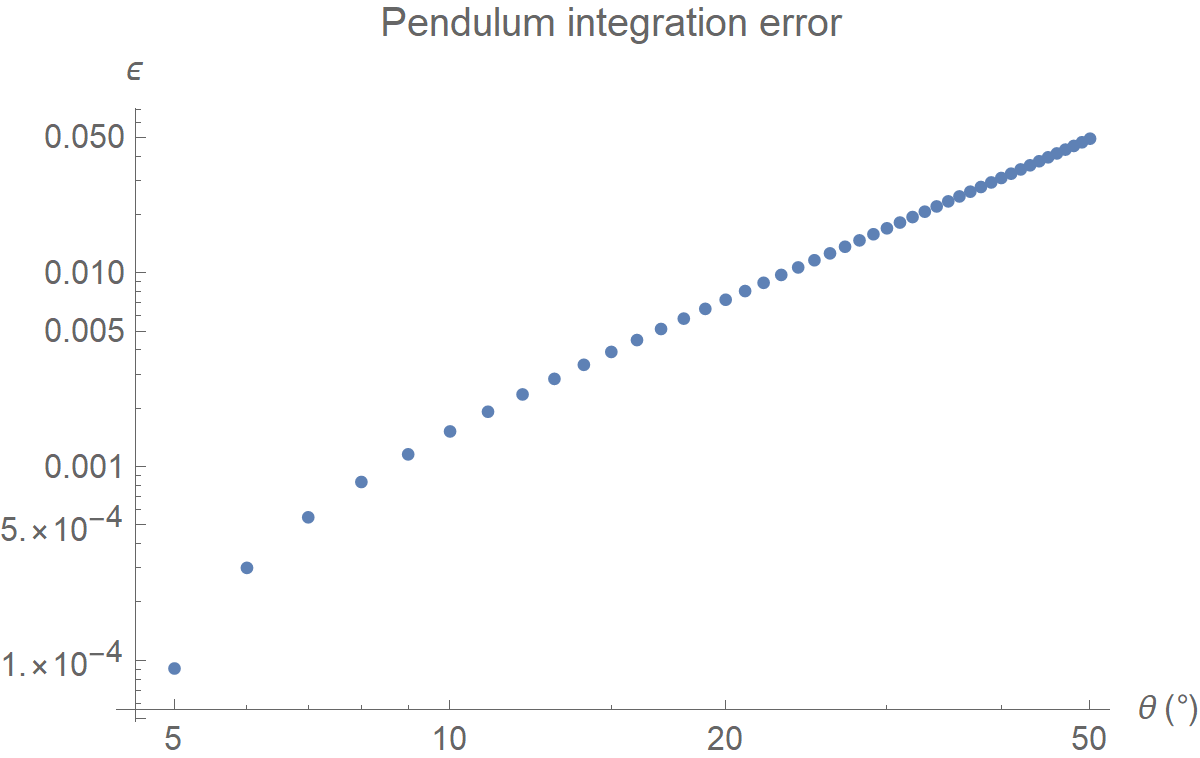
\includegraphics[width=5in]{homework2/pendulum.png}
    \caption{Caption}
    \label{fig:pendulum}
\end{figure}

\section{Conclusion}

\end{document}
